% Begin.....
\section{Server Information}\

\subsection{Hardware basic information}\

\begin{itemize}
    \item \textbf{Type:} DELL Precision 3660 Workstation
    \item \textbf{Service code:} 35K0L24
    \item \textbf{CPU:} 13th Gen Intel(R) Core(TM) i9-13900K
    \item \textbf{Video Card:} NVIDIA GeForce RTX 4090  Memory: 24G
    \item \textbf{Memory:} 128G
    \item \textbf{Hard disk 1:} nvme0n1 1T (NVMe SSD)
    \item \textbf{Hard disk 2:} sda 4T
\end{itemize}

\subsection{Login Address}
%\vspace{1cm}
\begin{itemize}
    \item \textbf{Server address:} 172.16.33.244
    \item \textbf{Admin User name:} Administrator, \textbf{Password:} hexing@2025
    \item \textbf{User name} : ems,\textbf{ Password:} sme8003
\end{itemize}

\section{AI Related System}\

\subsection{Ollama - AI local LLM inference server}\

How to \textbf{install} the ollama on Ubuntu ?
\vspace{0.5cm}
%\input{code/command}
%\begin{minted}[frame=single,framesep=1mm,breaklines=true]{bash}
%curl -L <https://ollama.com/download/ollama-linux-amd64.tgz> -o ollama-linux-amd64.tgz
%cd /home/user/tools/ollama
%gunzip ollama-linux-amd64.tgz
%tar xvf ollama-linux-amd64.tar
%cd ollama/bin
%./ollama serve
%\end{minted}

\begin{lstlisting}
# download the installation package
curl -L <https://ollama.com/download/ollama-linux-amd64.tgz> -o ollama-linux-amd64.tgz

# uncompress the package
cd /home/user/tools/ollama
gunzip ollama-linux-amd64.tgz
tar xvf ollama-linux-amd64.tar

# run the ollama service, also can configure to the system startup service
cd ollama/bin
./ollama serve
\end{lstlisting}

By typing in the browser\textbf{"http://172.16.33.244:11434"} to check if Ollama's service is working properly  

if display \textbf{"Ollama is running" }that means Ollama is running well.

%\colorline[red]{0.05pt}
\shortdashline

After\textbf{ “ollama pull”} command, can use \textbf{“ollama list” }to check the current models.

\begin{figure}[H]
    \begin{center}
        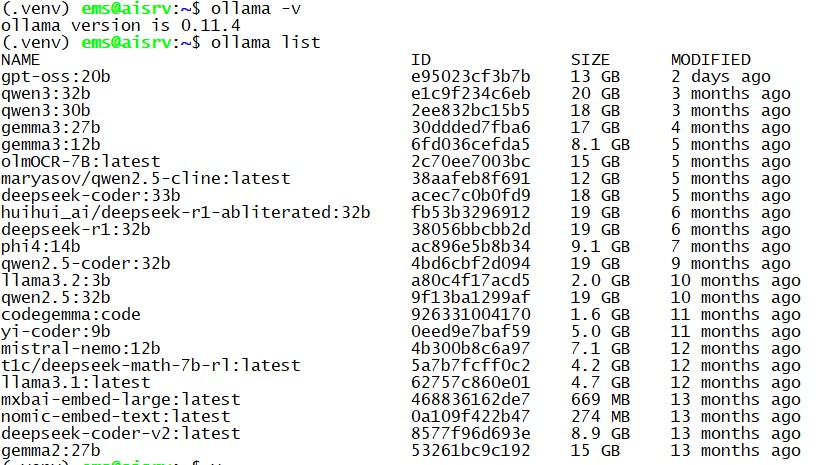
\includegraphics[width=.95\linewidth]{res/ollama_list.jpg}\\
        \caption{ All the available LLMs}\label{ollama_list}
    \end{center}
\end{figure} 

\shortdashline

By \textbf{"nvidia-smi"} to check video card information

\begin{figure}[H]
    \begin{center}
        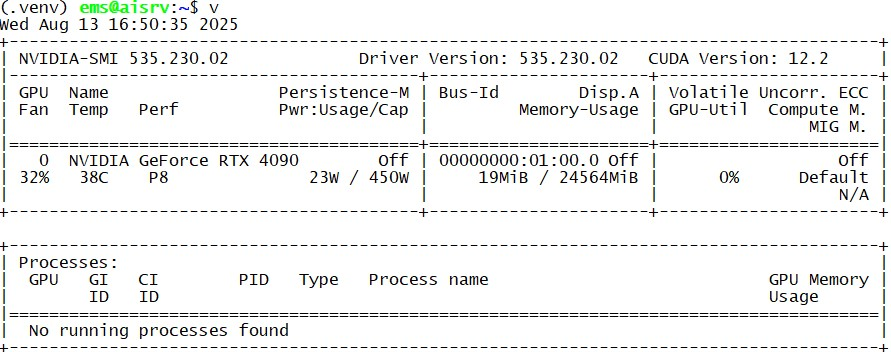
\includegraphics[width=.95\linewidth]{res/video_card_info.jpg}\\
        \caption{ video card information}\label{video_card_info}
    \end{center}
\end{figure} 

